\documentclass[fleqn, oneside, listof=totoc,% 
 bibliography=totoc, paper=A4]{scrartcl}[2007/12/24]
\addtokomafont{caption}{\normalsize}
\addtokomafont{captionlabel}{\bfseries}
\setcapindent{0em}
\usepackage{setspace}
\usepackage[utf8]{inputenc}
\usepackage[T1]{fontenc}
% \usepackage{lmodern}
\usepackage{mathptmx}
\usepackage{paralist}
\usepackage[american]{babel}
\usepackage{subfigure}
\usepackage{amsmath}
\usepackage{ellipsis}
\usepackage{lastpage}
\usepackage{microtype}
\usepackage[nottoc]{tocbibind}
\usepackage{booktabs}
\usepackage{tabularx}
\usepackage{amsfonts, amsthm}
\usepackage{appendix}
\usepackage[numbers,square, sort&compress]{natbib}
\usepackage{todonotes}
\usepackage{framed, color}
\usepackage{rotating, pdflscape, longtable}
\usepackage{graphicx}
\newcommand{\HRule}{\rule{\linewidth}{0.5mm}}
\usepackage[amssymb]{SIunits}
\usepackage{units}
\usepackage{amssymb}
\usepackage{color}
\usepackage{makeidx}
\usepackage{subfigure}
\usepackage{multirow}
\usepackage{multicol}
\usepackage{url}
\usepackage{attachfile}
\usepackage{mathtools}
%\usepackage[a4paper=true, pagebackref=true]{hyperref}
%\hypersetup{%
%    colorlinks=true, linktocpage=true, pdfstartpage=3, pdfstartview=FitV,%
%    % uncomment the following line if you want to have black links (e.g., for printing)
%    %colorlinks=false, linktocpage=false, pdfborder={0 0 0}, pdfstartpage=3, pdfstartview=FitV,%
%    breaklinks=true, pdfpagemode=UseNone, pageanchor=true, pdfpagemode=UseOutlines,%
%    plainpages=false, bookmarksnumbered, bookmarksopen=true, bookmarksopenlevel=1,%
%    hypertexnames=true, pdfhighlight=/O,%hyperfootnotes=true,%nesting=true,%frenchlinks,%
%    urlcolor=black, linkcolor=black, citecolor=black, %pagecolor=RoyalBlue,%
%    %urlcolor=Black, linkcolor=Black, citecolor=Black, %pagecolor=Black,%
%    pdftitle={Systems high-throughput repertoire analysis of  bone
%  marrow plasma cells of healthy and antigen-challenged mice},%
%    pdfauthor={Victor Greiff},%
%    pdfsubject={},%
%    pdfkeywords={HTRA, BMPCR, systems immunology},%
%    pdfcreator={pdfLaTeX},%
%    pdfproducer={LaTeX with hyperref}%
%  }

\newtheorem{thm}{Theorem}[section]
\newtheorem{cor}[thm]{Corollary}
\newtheorem{lem}[thm]{Lemma}

%\theoremstyle{definition}
\newtheorem{defin}[thm]{Definition}

\newcommand{\Mod}[1]{\ \mathrm{mod}\ #1}

\title{Supplemental Text}
\begin{document}

\section{Supplemental Text. Derivation of an analytical solution for the theoretical number of motifs within one CDR/FR region}
\label{sec:entr-relat-proofs}

\subsection{Objectives and motif definition}
\label{sec:objectives}


Our aim is to determine the number of possible structural interaction motifs for any motif
length. A given sequence motif is defined as follows:

\begin{itemize}
\item An amino acid is encoded as \textbf{X}.
\item A gap is encoded as integer $n$ where $n$ quantifies the length of the gap. 
\item Each motif starts and ends with an amino acid \textbf{X}.
\item There can be $>1$ amino acids in sequential positions but not $>1$ gaps.
\end{itemize}
Let us give two different definitions of motif length. By simply ``motif length'' we mean 
the number of \textbf{X}s in it plus the number of gaps, we note this lengths $L$. 
By ``amino acid length'', we mean the number of amino acids included in the sequence, 
i.e. the number of \textbf{X}s plus the sum of all gap lengths. Please, refer to the section \ref{sec:examples} for a few examples.

As the interaction sequence cannot exceed the size of the CDR/FR it is located in, we need to add one more constraint:
\begin{itemize}
\item The amino acid length of the motif is not bigger then a predefined number.
\end{itemize}

Let us denote the number of unique motifs of lengths $L$ and amino acid length $A$ as $\mathrm{N}_{L, A}$ 
and the number of unique motifs of length $L$ with amino acid length \textit{not exceeding} $A$ as $\bar{\mathrm{N}}_{L, A} = \sum_{A_1=L}^A \mathrm{N}_{L, A_1}$


\subsection{Examples}
\label{sec:examples}

To derive a formula for $\mathrm{N}_{L,A}$, we inspect a few examples first for intuition purposes. 

\begin{align*}
L = 1,& \: A = 1 &&\rightarrow \mathbf{X} &\rightarrow \mathrm{N}_{1, 1} = 1\\
L = 2,& \: A = 2 &&\rightarrow \mathbf{XX} &\rightarrow \mathrm{N}_{2, 2} = 1\\
L = 3,& \: A = 3 &&\rightarrow \mathbf{XXX}, \mathbf{X}1 \mathbf{X} &\rightarrow \mathrm{N}_{3, 3} = 2\\
L = 3,& \: A = n > 3 &&\rightarrow \mathbf{X}k\mathbf{X}, \;\; (k = n - 2) &\rightarrow \mathrm{N}_{3, n} = 1\\
L = 4,& \: A = 4 &&\rightarrow \mathbf{XXXX}, \mathbf{X}1\mathbf{XX}, \mathbf{XX}1\mathbf{X} &\rightarrow \mathrm{N}_{4, 4} = 3\\
L = 4,& \: A = n > 4 &&\rightarrow \mathbf{X}k\mathbf{XX}, \mathbf{XX}k\mathbf{X} \;\; (k = n - 3)  &\rightarrow \mathrm{N}_{4, n} = 2\\
L = 5,& \: A = 5 &&\rightarrow \mathbf{XXXXX}, \mathbf{X}1\mathbf{XXX}, \mathbf{XX}1\mathbf{XX}, \mathbf{XXX}1\mathbf{X}, \mathbf{X}1\mathbf{X}1\mathbf{X} &\rightarrow \mathrm{N}_{5, 5} = 5\\
L = 5,& \: A = n > 5 &&\rightarrow \mathbf{X}k\mathbf{XXX}, \mathbf{XX}k\mathbf{XX}, \mathbf{XXX}k\mathbf{X}, \mathbf{X}k_1\mathbf{X}k_2\mathbf{X} 
 &\rightarrow \mathrm{N}_{5, n} = n-1\\
\end{align*}
In the last line, $k = n - 4$ and $k_1 + k_2 = n-3$. Let us clarify this last line: there are only $3$ motifs with a single gap, 
but if there are two gaps, their lengths can vary:
$k_1 = 1, k_2 = n-4$;\;\; $k_1 = 2, k_2 = n - 5, \; \dots \;,$ so that we have $n-4$ double-gapped motifs in total.

\subsection{General formula}
Now we can proceed to derive a general formula for $\mathrm{N}_{L, A}$. Let us note the number of $\mathbf{X}$s in a motif
 as $n_x$ and the number of gaps as $n_g$. 
 We can count the motifs for fixed $n_x$ and $n_g$ and then 
 we will just have to sum the results over all $n_x  + n_g = L$. 
 Thus, we have $n_x$ $\mathbf{X}$s and $n_x - 1$ slots for gaps -- 
 between any two neighbouring $\mathbf{X}$s there can be a gap. 
 First, we have to choose $n_g$ slots: the number of ways to do this is 
$$n_x - 1 \choose n_g$$
 Now we have $n_g$ gaps of total amino acid length $A - n_x$, and we need to distribute 
 the lengths between the gaps. In other words, we need to split the number $A - n_x$ 
 into a sum of $n_g$ nonzero terms. The number of ways to do this is the number of $n_g$\textit{-compositions} of $A - n_x$,
 which equals
 $$A - n_x - 1 \choose n_g - 1$$
Now we can write down the formula for $\mathrm{N}_{L, A}$ as 
$$\mathrm{N}_{L,A} = \sum_{n_g + n_x = L, n_g \le n_x - 1} {n_x - 1 \choose n_g} {A - n_x - 1 \choose n_g - 1}$$
We did not take into account the all-$\mathbf{X}$ case, so for $A=L$ we should have
$$\mathrm{N}_{L,L} = 1 + \sum_{n_g + n_x = L, n_g \le n_x - 1} {n_x - 1 \choose n_g} {A - n_x - 1 \choose n_g - 1}$$
Similarly, the formula for $\bar{\mathrm{N}}_{L, A}$ is 
$$\bar{\mathrm{N}}_{L,A} = \sum_{A_1 = L}^A \mathrm{N}_{L,A_1} = 1 + \sum_{A_1 = L}^A \; \sum_{n_g + n_x = L, n_g \le n_x - 1} {n_x - 1 \choose n_g} {A_1 - n_x - 1 \choose n_g - 1}$$

Figures~\ref{fig:motifs_count_by_region}~and~\ref{fig:total_motifs_count} show the growth of $\bar{\mathrm{N}}_{L,A}$ for $L$ in $1, ..., 10$. We set 10 as maximum motif length based on our observations (see Fig. 2B in the main text). 


\begin{figure}[!ht]
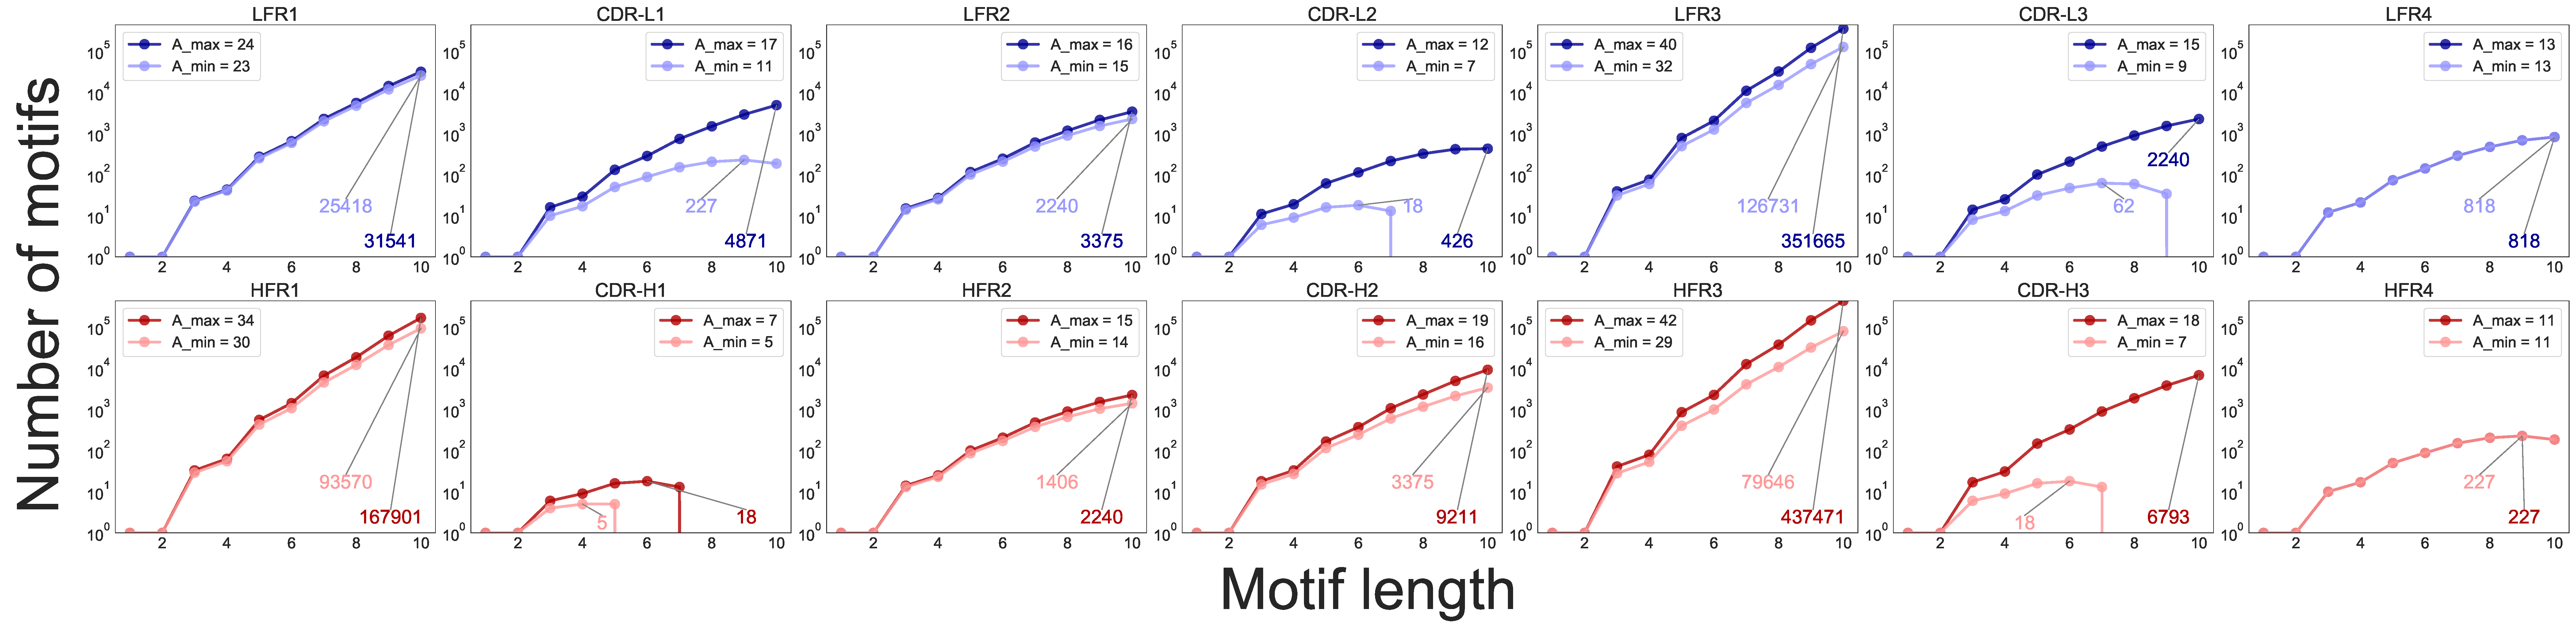
\includegraphics[width=0.99\textwidth]{figures/motifs_number_fig.pdf}
\caption[]{The number of unique motifs (Y axis) for a given motif length (X axis) that could be located in a certain FR/CDR (see possible FR/CDR lengths in Supplementary Table S1). The amino acid length of the motifs is bounded by the minimum and maximum possible region length (Supplementary Table S1).}
\label{fig:motifs_count_by_region} 
\end{figure}
\begin{figure}[!ht]
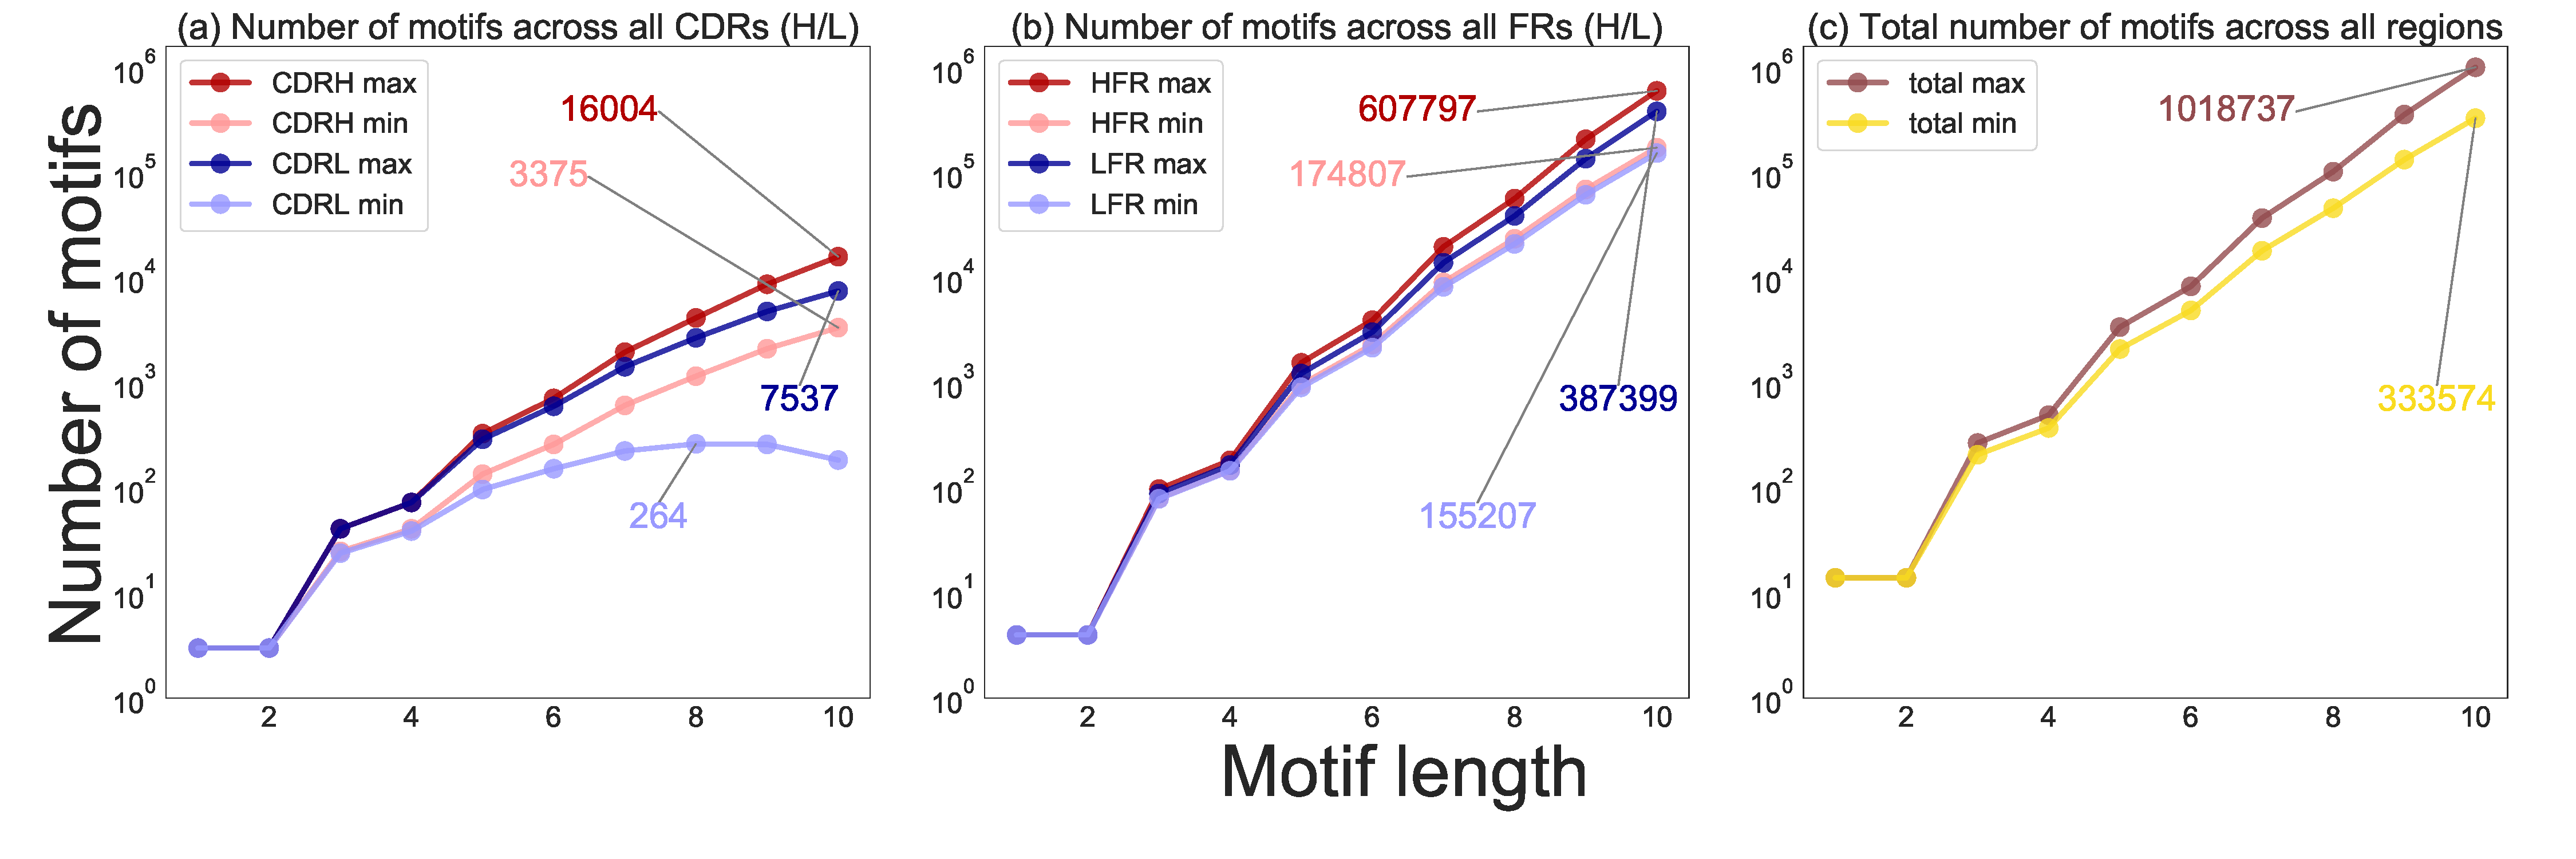
\includegraphics[width=0.99\textwidth]{figures/total_motifs_number_fig.pdf}
\caption[]{The total number of unique motifs (Y axis) for a given length (X axis) across all CDR-Ls and CDR-Hs \textbf{(a)}, across all LFRs and HFRs \textbf{(b)}, across all regions \textbf{(c)}.}
\label{fig:total_motifs_count}
\end{figure}

















\end{document}
